\chapter{Background}\label{chapter:background}
This chapter shall provide a high-level introduction to the cryptographical and mathematical tools used to implement attribute-based encryption in this thesis. For further reference, please refer to % TODO


\begin{figure} \centering
    \begin{subfigure}{.7\textwidth}
        \begin{tikzpicture}
            \draw[->] (0, 0) node [anchor=east] {m} -- ++(1, 0) node (encrypt) [anchor=west, draw] {Encrypt};
            \path (encrypt.north) -- +(0, 0.3) pic [anchor=west, scale=0.1, fill=blue] {key};
            \draw[->] (encrypt.east) -- ++(2, 0) node [anchor=south] {c} -- ++(2,0) node (decrypt) [anchor=west, draw] {Decrypt};
            \path (decrypt.north) -- +(0, 0.3) pic [anchor=west, scale=0.1, fill=blue] {key};
            \draw[->] (decrypt.east) -- ++(1,0) node [anchor=west] {m'};
        \end{tikzpicture}
        \caption{Symmetric Encryption} \label{fig:keys-symmetric}
    \end{subfigure}
    \\
    \vspace{0.5cm}
    \begin{subfigure}{.7\textwidth}
        \begin{tikzpicture}
            \draw[->] (0, 0) node [anchor=east] {m} -- ++(1, 0) node (encrypt) [anchor=west, draw] {Encrypt};
            \path (encrypt.north) -- +(0, 0.3) pic [anchor=west, scale=0.1, fill=green] {key};
            \draw[->] (encrypt.east) -- ++(2, 0) node [anchor=south] {c} -- ++(2,0) node (decrypt) [anchor=west, draw] {Decrypt};
            \path (decrypt.north) -- +(0, 0.3) pic [anchor=west, scale=0.1, fill=red] {key};
            \draw[->] (decrypt.east) -- ++(1,0) node [anchor=west] {m'};
        \end{tikzpicture}
        \caption{Asymmetric Encryption} \label{fig:keys-asymmetric}
    \end{subfigure}
    \\ 
    \vspace{0.5cm}
    \begin{subfigure}{.7\textwidth}
        \begin{tikzpicture}[sibling distance=4mm, level distance=3mm]
            \draw[->] (0, 0) node [anchor=east] {m} -- ++(1, 0) node (encrypt) [anchor=west, draw] {Encrypt};
            
            \scoped{
                \tikzstyle{every node}=[fill, circle, draw, inner sep=0.5mm];
                \tikzstyle{level 2}=[sibling distance=1.5mm];
                \fill[olive] (encrypt.north) -- ++(0, 0.7) node [anchor=south] {} child {node {} child {node {}} child {node {}} child {node {}}} child { node {} child {node {}}};
            };
            \draw[->] (encrypt.east) -- ++(2, 0) node [anchor=south] {c} -- ++(2,0) node (decrypt) [anchor=west, draw] {Decrypt};
            \path (decrypt.north) -- +(0, 0.3) pic [anchor=west, scale=0.1, fill=magenta] {key};
            \draw[->] (decrypt.east) -- ++(1,0) node [anchor=west] {m'};
        \end{tikzpicture}
        \caption{Attribute-Based encryption} \label{fig:keys-abe}
    \end{subfigure}
    \caption{Keys used for encryption and decryption in different classes of encryption schemes}
\end{figure}

\section{Classic Symmetric and Asymmetric Cryptography}
Today's conventional cryptography knows two main classes of cryptosystems: \emph{Symmetric} or \emph{Private-Key systems} and \emph{Asymmetric} or \emph{Public-Key systems}.
The main difference lies in their use of encryption and decryption keys:

In \emph{symmetric} systems, the key used for encryption and decryption is identical.
That is, a user \emph{Alice} encrypting a message to send to another user \emph{Bob} will encrypt the message using a key $k$ that she had agreed on with Bob beforehand.
When he receives the encrypted message, Bob will use the same key $k$ to decrypt it. See Figure~\ref{fig:keys-symmetric}.

In \emph{asymmetric} systems, on the other hand, the keys used for encryption and decryption differ.
When Alice encrypts a message with key $k_{enc}$, she will not be able to encrypt it again.
Instead, when Bob receives the encrypted message, he will use a different key $k_{dec}$ to decrypt it. See Figure~\ref{fig:keys-asymmetric}.
Thus, in symmetric systems, keys always come in \emph{pairs} of an \emph{encryption key} $k_{enc}$ and a \emph{decryption key} $k_{dec}$.
Because $k_{enc}$ can not be used to decrypt messages meant for Bob, there is no harm to making it publicly available.
For example, he might put it up on his website for anyone wishing to send him an encrypted message to download. This is why $k_{enc}$ is also often called the \emph{public key} and $k_{dec}$ the \emph{private key}.

Asymmetric cryptosystems make secure communication among a large group of participants much easier:
Consider $n$ participants wanting to communicate securely using a symmetric system.
Each participant would need to share a unique secret key with each of the other participants, requiring a total of $\frac{n(n-1)}{2}$ keys. In the asymmetric setting, one key per participant is sufficient:
The same public key may be shared with the whole group, as the private key remains private anyway. This reduces the total number of keys to $n$.

Another problem remains, however: Encrypting a single message to a large number of participants requires encrypting it with everyone's public key separately.
For a large number of recipients, this is inefficient.
So, for example, to encrypt a message for all students of a certain university, we'd need to obtain each student's public key and encrypt the message with each key separately.

Even worse, what if we want to encrypt data for any student of said university, even if they \emph{haven't joined the university yet}.
In this case, our only option using classic public-key cryptography would be to have some trusted instance encrypt the data for any new student after they joined the university.
Attribute-Based encryption solves this problem much more nicely. 

\section{Attribute-Based Encryption}

Attribute-Based Encryption Schemes (ABE schemes) are asymmetric in the sense that different keys are used for encryption and decryption.
However, in constrast to classic asymmetric systems, the 'public key' used for encryption is not attached to an identity, but to certain attributes defined by the system.
This is represented by a tree of attributes in Figure~\ref{fig:keys-abe}.


\subsection{KP-ABE and CP-ABE}
ABE schemes can further be divided into \emph{Key-Policy} and \emph{Ciphertext-Policy} schemes (KP-ABE and CP-ABE, respectively).
In KP-ABE, the ciphertext is associated with a set of attributes, and the key is associated with an access structure.
CP-ABE works the other way around, so the key is associated with a set of attributes and the ciphertext is encrypted under an access structure.

In both cases, a ciphertext can be decrypted if and only if the set of attributes specified in one part satisfy the access policy associated with the other part.



\subsection{Components of an ABE scheme}

With respect to ABE, we say that a ciphertext is \emph{encrypted under an access structure} (\emph{under a set of attributes}, respectively) if it has been encrypted using the public key derived from the access structure (set of attributes, resp.).
Because the public key w.r.t. some access structure (set of attributes, resp.) can be derived by anyone, private keys are usually referred to as just \emph{keys}.

An Attribute-Based Encryption scheme (ABE scheme) consists of the following four algorithms: 
\begin{itemize}
    \item \emph{Setup}. Run once by the central trusted authority (key generation center). Sets up the system and outputs a public master key $PK$ and a private master secret $s$.
    \item \emph{KeyGen(PK, s, $\omega$)}. Run exclusively by the trusted authority. For a given set of attributes (CP-ABE) or access structure (KP-ABE) $\omega$, uses the master secret $s$ to generate a private key $k$ corresponding to the given access structure.
    \item \emph{Encrypt(PK, m, $\omega$)}. Run by any participant of the system. On input of a plaintext message $m$ and an access structure (CP-ABE) or set of attributes (KP-ABE) $\omega$, outputs a ciphertext $c$
    \item \emph{Decrypt(c, k)}. Run by any participant holding a private key generated by \emph{KeyGen}. On input of a ciphertext $c$ created by \emph{Encrypt} and a key $k$ generated by \emph{KeyGen}, it outputs a correctly decrypted message if and only if
    \begin{itemize}
        \item in the case of CP-ABE: the access structure under which $m$ was encrypted is satisfied by the set of attributes under which $k$ was created
        \item in the case of KP-ABE: the set of attributes under which $m$ was encrypted satisfies the access structure under which $k$ was created.
    \end{itemize}
\end{itemize}

\section{Shamir's Secret Sharing}
This secret sharing scheme based on polynomial interpolation was first introduced by Adi Shamir in 1979~\cite{shamir_how_1979}.
It allows a secret $s$, which is generally just a number, to be shared among a number of $n$ participants.
The shares are computed such that $s$ can be reconstructed if, and only if, at least $k$ participants meet and combine their shares.
Such a theme is then called a $(k,n)$-threshold scheme.~\cite{shamir_how_1979}

Shamir's scheme makes use of a property of polynomials: A polynomial of degree $d$ is unambiguously determined by $d+1$ points $(x_i, y_i)$.
In other words, any polynomial of degree $d$ can be unambiguously interpolated (reconstructed) from $d+1$ distinct points.
Thus, if we hide our secret in a polynomial $p(x)$ of degree $d$ and give out secret shares as $(x, p(x))$ with $x = 1, 2, 3, \dots$, we can use $d+1$ shares to reconstruct $p(x)$ and by that the secret.\cite{shamir_how_1979}

\begin{figure}
    \centering
    \begin{tikzpicture}
        \begin{axis} [axis lines=center, xlabel=$x$, ylabel=$p(x)$]
            \addplot [domain=-0.1:5.05, smooth, thick, color=red] { \PolynomialSSS(x)};
            \fill (axis cs:0,\PolynomialSSS(0)) circle [radius=2pt] node [right] {(0,s)};
            \fill (axis cs:1,\PolynomialSSS(1)) circle [radius=2pt] node [right] {(1,$p(1)$)};
            \fill (axis cs:2,\PolynomialSSS(2)) circle [radius=2pt] node [right] {(2,$p(2)$)};
            \fill (axis cs:3,\PolynomialSSS(3)) circle [radius=2pt] node [above] {(3,$p(3)$)};
            \fill (axis cs:4,\PolynomialSSS(4)) circle [radius=2pt] node [right] {(4,$p(4)$)};
            \fill (axis cs:5,\PolynomialSSS(5)) circle [radius=2pt] node [left] {(5,$p(5)$)};
          \end{axis}
    \end{tikzpicture}
    \caption{Example for a $(5, 4)$-threshold scheme with $s=12$ and $p(x) = 12 + 7x - 6x^2 + x^3$. As $p(x)$ has degree three, at least four of the five shares are required to reconstruct $s$.}
    \label{fig:sss}
\end{figure}

That is, to create a simple $(k, n)$-threshold scheme to share a secret $s$, do the following:~\cite{shamir_how_1979}
\begin{enumerate}
    \item Pick coefficients $a_1, ..., a_{k-1}$ at random 
    \item Set $a_0 = s$. This results in the polynomial $p(x) = a_0 + a_1x + \cdots + a_{k-1}x^{k-1}$. Note that $p(0) = s$.
    \item The secret shares are $(1, p(1)), (2, p(2)), \dots, (n, p(n))$. Give one to each participant.
\end{enumerate}

To reconstruct the secret from any subset of $k$ shares, simply interpolate the polynomial $p(x)$ and evaluate $p(0) = s$~\cite{shamir_how_1979}.
See also Figure~\ref{fig:sss} for illustration.

The polynomial can be interpolated unambiguously if at least $k$ points are known, because it has degree $k-1$.
If only $k-1$ points (or less) are known, there are infinitely many ways to construct a polynomial that passed through all $k-1$ points.
Therefore, then there are also infinitely many possibilities for $s$.~\cite{shamir_how_1979}



\section{Elliptic Curves}

The mathematics of modern cryptosystems (including, but not limited to ABE) work on a great variety of mathematical structures, and elliptic curves are just one of them.
They have become very popular since their discovery by \emph{citation needed} in \emph{year needed} because they provide an equivalent security level at shorter key length and smaller computational cost than other systems (e.g. based on RSA) \cite{katz_introduction_2015}.
Exact definitions and notations differ, these are taken from the textbook \emph{Introduction to Modern Cryptogaphy} by Katz and Lindell~\cite{katz_introduction_2015}.

Elliptic curves (over finite fields) are defined by equations of the following form, where $p \leq 5$ prime: \cite{katz_introduction_2015}
\begin{equation}
    y^2 = x^3 + a x + b \pmod{p}
\end{equation}
$a$ and $b$ are the curve parameters, and it is required that $4a^2 + 27b^2 \neq 0 \pmod{p}$ (this makes sure there are no repeated roots).\cite{katz_introduction_2015}

Then, the elliptic curve $E(\mathbb{Z}_p)$ is the set of coordinates $(x, y) \in \mathbb{Z}_p^2$ that satisfies the equation above. 
A special value $\mathcal{O}$ is added to denote the \emph{point at infinity}. \cite{katz_introduction_2015}
\begin{equation}
    E(\mathbb{Z}_p) := \{(x, y) | x,y \in \mathbb{Z}_p \text{ and } y^2 = x^3 + a x + b \text{ mod } b\} \cup \{\mathcal{O}\}
\end{equation}

\subsection{Point Addition}
Now, it is possible to show that every line intersecting a curve $E(\mathbb{Z}_p)$ intersects it in exactly three points, if you (1) count tangential intersections double and (2) count any vertical line as intersecting the curve in the point at infinity $\mathcal{O}$.
Therefore, $\mathcal{O}$ can be thought of as sitting 'above' the end of the y-axis.\cite{katz_introduction_2015}

Using this intersecting line, we can define an operation on curve points called \emph{(point) addition} and written using $+$: \cite{katz_introduction_2015}

\begin{itemize}
    \item $\mathcal{O}$ is the identity, i.e. for any $P \in E(\mathbb{Z}_p)$, $P + \mathcal{O} = \mathcal{O} = \mathcal{O} + P$ 
    \item For two points $P_1, P_2 \neq \mathcal{O}$, their sum $P_1 + P_2$ is evaluated by drawing the line through $P_1$ and $P_2$ (if $P_1 = P_2$, draw a tangential line). 
        This line will intersect the curve in a third point, $P_3 = (x_3, y_3)$.
        Then the result of the addition is $P_1 + P_2 = (x_3, -y_3)$, i.e. $P_3$ is reflected in the $x$-axis.
        If $P_3 = \mathcal{O}$, then the result of the addition is $\mathcal{O}$.
\end{itemize}

\begin{figure}
    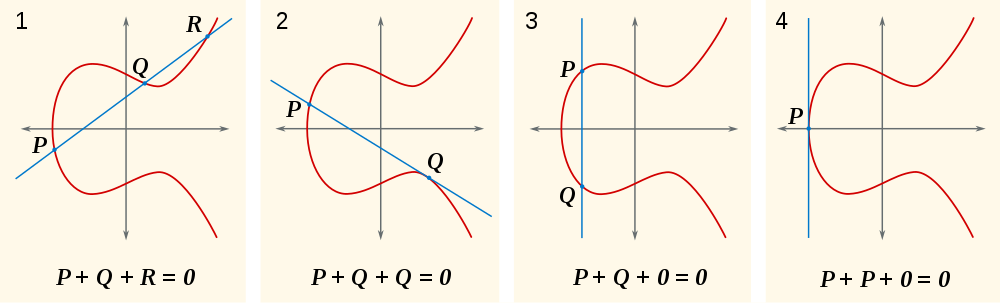
\includegraphics[width=\textwidth]{figures/ecc_point_addition.png}
    \caption{Elliptic Curve point addition\\(Image by \href{https://commons.wikimedia.org/wiki/File:ECClines.svg}{SuperManu}, licensed under \href{https://creativecommons.org/licenses/by-sa/3.0/deed.en}{Creative Commons}.)}
    \label{fig:ecc-point-addition}
\end{figure}

In addition, we define multiplication of a point $P \in E(\mathbb{Z}_p)$ with a scalar $n \in \mathbb{N}$ as follows:
\begin{equation}
    n \cdot P = \underbrace{P + P + \cdots + P}_{n \text{ times}}
\end{equation}
 
That is, the product of a scalar with a point is again a point on our curve.
\\

\subsection{Groups on Elliptic Curves}
For any point $P = (x,y)$, there is unique inverse $-P = (x, -y)$.
In addition associativity holds (i.e. for all $P_1, P_2, P_3 \in E(\mathbb{Z}_p)$, $(P_1 + P_2) + P_3 = P_1 + (P_2 + P_3))$.
Thus, $E(\mathbb{Z}_q)$ with point addition is a group. \cite{katz_introduction_2015}

Of particular interest to cryptography are \emph{cyclic} groups on elliptic curves. 
A (multiplicative) group $\mathbb{G}$ is cyclic if there is an element $g \in \mathbb{G}$ that generates $\mathbb{G}$, i.e. $G = \langle g \rangle = \{g^n | n \in \mathbb{Z}\}$.
Translated to our (additive) groups on elliptic curves, this means that there is a generator point $P \in E(\mathbb{Z}_p)$, such that every point $Q \in E(\mathbb{Z}_p)$ can be written as $Q = nP$ with some $n \in \mathbb{N}$.

In particular, if a group has prime order (i.e. the number of points $\#E(\mathbb{Z}_p)$ on a curve is prime), all points except $\mathcal{O}$ are generators.
This follows from the fact that for any point $P \in E(\mathbb{Z}_p)$, its order $\text{ord}(P) = | \langle P \rangle |$ must divide the group order.
A prime has exactly two divisors: One (the order of $\mathcal{O}$) and itself (the order of all other points).

These cyclic elliptic curve groups (or, cyclic subgroups of non-cyclic elliptic curves) are exactly the groups we are interested in for doing actual cryptography. See also \cite[p.~321]{katz_introduction_2015}.

\subsection{Hardness Assumptions}

Most ECC schemes are build upon three hardness assumptions: The Discrete Logarithm Problem (DLP), the Decisional Diffie-Hellman Problem (DDHP) and the Computational Diffie-Hellman Problem (CDHP).
Given an additive, cyclic group $\mathbb{G}$ with $P \in \mathbb{G}$ a generator, they are stated as follows:
\\

\emph{Discrete Logarithm Problem.} Given an arbitrary $Q \in \mathbb{G}$, compute an $n \in \mathbb{N}$ such that $n P = Q$. % n from Zq?

\emph{Computational Diffie-Hellman Problem.} Given the triple $(P, aP, bP)$ where $a, b \in \mathbb{N}$ chosen uniformly at random, compute $abP$.

\emph{Decisional Diffie-Hellman Problem.} Given two triples $(aP, bP, abP)$ and $(aP, bP, Q)$ where $a, b \in \mathbb{N}$ and $Q \in \mathbb{G}$ chosen uniformly at random, distinguish between the two.
\\

Now, the hardness \emph{assumption} is that, for some groups, these problems are hard to solve, i.e. solving them requires so much time and computational power that it is infeasible.
From this, we can build secure asymmetric encryption schemes.

These three problems might all be assumed to be \emph{hard}, but that doesn't mean they are equally so:
If, in a certain group $\mathbb{G}$, the DLP problem is easy, so is CDHP: Just compute $a$ and $b$, and then use them to calculate $abP$.
And if CDHP is easy w.r.t some $\mathbb{G}$, so is DDHP: Just compute $abP$, and compare the third element of each tuple.
The inverse is not generally true, i.e. there are groups in which DLP and CDHP are hard to solve, even though DDHP is easy to solve.
In that sense, DLP is the hardest and DDHP the easiest of the three. \cite{katz_introduction_2015} (TODO find out if this is true. \cite{menezes_introduction_2009})

\subsection{Bilinear Pairings}
\subsubsection{Introduction}
The final primitive needed for pairing-based encryption schemes are bilinear pairings. These are functions mapping two points on (possibly different) elliptic curves to elements of a finite field (\emph{not} another point on a curve).\cite{blake_advances_2005}

Let $n \in \mathbb{N}_0$, $\mathbb{G}_1$ denote an additive abelian group of order $n$ with generator $P$ and identity $\mathcal{O}$. 
Let $\mathbb{G}_T$ be another group of order $n$, this time written multiplicatively with generator $g$ and identity $1$.
A \emph{bilinear pairing} then is a function $e: \mathbb{G}_1 \times \mathbb{G}_1 \rightarrow \mathbb{G}_T$ with the following properties:
\begin{itemize}
    \item \emph{Bilinearity.} For all $Q_1, Q_2, Q_3 \in \mathbb{G}_1$, $e(Q_1+Q_2, Q_3) = e(Q_1,Q_3)+e(Q_2,Q_3)$ and $e(Q_1, Q_2+Q_3)=e(Q_1,Q_2)+e(Q_1,Q_3)$
    \item \emph{Non-Degeneracy.} $e(P,P) \neq 1$
\end{itemize}

Using a bilinear pairing with a group $\mathbb{G}_T$ where the DLP is easy to solve, the DLP in $\mathbb{G}_1$ can also be solved easily:
To find $n$ such that $Q = nP$, compute $e(P,Q) = e(P, nP) = e(P, \underbrace{P+\cdots+P}_{n \text{ times}}) = \underbrace{e(P,P) \cdots e(P,P)}_{n \text{ times}} = e(P,P)^n$.
Thus, the discrete logarithm of $Q$ with respect to $P$ is the discrete logarithm of $e(P,Q)$ with respect to $g = e(P,P) \in \mathbb{G}_T$.~\cite{menezes_introduction_2009}

\subsubsection{Bilinear Hardness Assumption}

Since the DLP can be easy to solve using pairings, we need to adapt our hardness assumption. Therefore, we define

The \emph{Bilinear Diffie-Hellman Problem} (BDHP): Given $P, aP, bP, cP$ with $a,b,c \in \{1,\dots,n-1\}$ chosen randomly, compute $e(P, P)^{abc}$.~\cite{menezes_introduction_2009}

If the BDHP is hard for a pairing $e$ on groups $\mathbb{G}_1 \text{ and } \mathbb{G}_T$, this implies that the DLP is hard in both $\mathbb{G}_1 \text{ and } \mathbb{G}_T$.~\cite{menezes_introduction_2009}

\section{Different ABE schemes for use in Embedded Devices}
